
\subsection*{1.}

Le lait de brebis est représenté par un secteur de \(60^\circ\) : sa proportion est donc de \(\dfrac{60}{360} = \dfrac{1}{6}\) ;

Le lait de chèvre est représenté par un secteur de \(90^\circ\) : sa proportion est donc de \(\dfrac{90}{360} = \dfrac{1}{4}\) ;

Le lait de vache est représenté par un secteur de \(360 - (60 + 90) = 360 - 150 = 210^\circ\) : sa proportion est donc de \(\dfrac{210}{360} = \dfrac{7}{12}\).

On a \( P_C(A) = 0{,}6 \) et \( P(B) = \dfrac{1}{6} \).


\subsection*{2.}

On peut dresser un arbre pondéré de probabilités :

\begin{center}
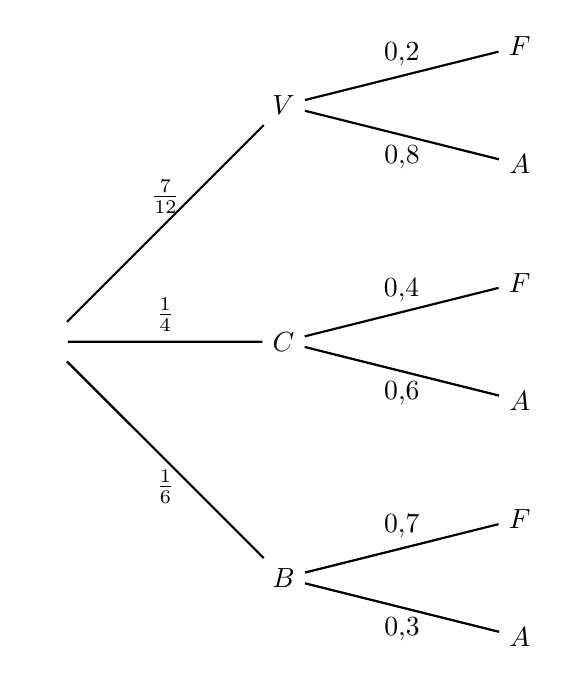
\begin{tikzpicture}[thick, scale=1.5]
\node (P_-1_0) at (-2,-2.5) {$\phantom{A}$};
\node (P_0_0) at (0,-0.5) {$V$};
\draw (P_-1_0) -- (P_0_0) node[midway, above] {$\frac{7}{12}$};
\node (P_1_0) at (2,-0) {$F$};
\draw (P_0_0) -- (P_1_0) node[midway, above] {$0{,}2$};
\node (P_1_1) at (2,-1) {$A$};
\draw (P_0_0) -- (P_1_1) node[midway, below] {$0{,}8$};
\node (P_0_2) at (0,-2.5) {$C$};
\draw (P_-1_0) -- (P_0_2) node[midway, above] {$\frac14$};
\node (P_1_2) at (2,-2) {$F$};
\draw (P_0_2) -- (P_1_2) node[midway, above] {$0{,}4$};
\node (P_1_3) at (2,-3) {$A$};
\draw (P_0_2) -- (P_1_3) node[midway, below] {$0{,}6$};
\node (P_0_4) at (0,-4.5) {$B$};
\draw (P_-1_0) -- (P_0_4) node[midway, below] {$\frac16$};
\node (P_1_4) at (2,-4) {$F$};
\draw (P_0_4) -- (P_1_4) node[midway, above] {$0{,}7$};
\node (P_1_5) at (2,-5) {$A$};
\draw (P_0_4) -- (P_1_5) node[midway, below] {$0{,}3$};
\end{tikzpicture}
\end{center}

Calculons les probabilités :
\[
P(V \cap A) = P(V) \times P_V(A) = \dfrac{7}{12} \times 0{,}8 = \dfrac{5{,}6}{12} = \dfrac{1{,}4}{3} = \dfrac{7}{15},
\]
\[
P(C \cap A) = P(C) \times P_C(A) = \dfrac{1}{4} \times 0{,}6 = \dfrac{0{,}6}{4} = 0{,}15,
\]
\[
P(B \cap A) = P(B) \times P_B(A) = \dfrac{1}{6} \times 0{,}3 = \dfrac{0{,}3}{6} = 0{,}05.
\]
D'après la loi des probabilités totales :
\begin{align*}
P(A) &= P(V \cap A) + P(C \cap A) + P(B \cap A) \\
&= \dfrac{7}{15} + 0{,}15 + 0{,}05 \\
&= \dfrac{7}{15} + 0{,}20 \\
&= \dfrac{7}{15} + \dfrac{3}{15} \\
&= \dfrac{10}{15} = \dfrac{2}{3}.
\end{align*}

\subsection*{3.}

On a :
\[
P_A(V) = \frac{P(V \cap A)}{P(A)} = \frac{\dfrac{7}{15}}{\dfrac{2}{3}} = \frac{7 \times 3}{15 \times 2} = \frac{21}{30} = \dfrac{7}{10},
\]
soit \(0{,}7\) à \(10^{-3}\) près.

